%Version 3 October 2023
% See section 11 of the User Manual for version history
%
%%%%%%%%%%%%%%%%%%%%%%%%%%%%%%%%%%%%%%%%%%%%%%%%%%%%%%%%%%%%%%%%%%%%%%
%%                                                                 %%
%% Please do not use \input{...} to include other tex files.       %%
%% Submit your LaTeX manuscript as one .tex document.              %%
%%                                                                 %%
%% All additional figures and files should be attached             %%
%% separately and not embedded in the \TeX\ document itself.       %%
%%                                                                 %%
%%%%%%%%%%%%%%%%%%%%%%%%%%%%%%%%%%%%%%%%%%%%%%%%%%%%%%%%%%%%%%%%%%%%%

%%\documentclass[referee,sn-basic]{sn-jnl}% referee option is meant for double line spacing

%%=======================================================%%
%% to print line numbers in the margin use lineno option %%
%%=======================================================%%

% \documentclass[lineno,sn-basic]{sn-jnl}% Basic Springer Nature Reference Style/Chemistry Reference Style

%%======================================================%%
%% to compile with pdflatex/xelatex use pdflatex option %%
%%======================================================%%

\documentclass[pdflatex,sn-basic, Numbered]{sn-jnl}% Basic Springer Nature Reference Style/Chemistry Reference Style

%%Note: the following reference styles support Namedate and Numbered referencing. By default the style follows the most common style. To switch between the options you can add or remove �Numbered� in the optional parenthesis.
%%The option is available for: sn-basic.bst, sn-vancouver.bst, sn-chicago.bst%

% \documentclass[sn-nature]{sn-jnl}% Style for submissions to Nature Portfolio journals
% \documentclass[sn-basic]{sn-jnl}% Basic Springer Nature Reference Style/Chemistry Reference Style
% \documentclass[sn-mathphys-num]{sn-jnl}% Math and Physical Sciences Numbered Reference Style
%%\documentclass[sn-mathphys-ay]{sn-jnl}% Math and Physical Sciences Author Year Reference Style
% \documentclass[sn-aps]{sn-jnl}% American Physical Society (APS) Reference Style
%\documentclass[sn-vancouver,Numbered]{sn-jnl}% Vancouver Reference Style
%%\documentclass[sn-apa]{sn-jnl}% APA Reference Style
%%\documentclass[sn-chicago]{sn-jnl}% Chicago-based Humanities Reference Style

%%%% Standard Packages
%%<additional latex packages if required can be included here>

\usepackage{graphicx}%
\usepackage{multirow}%
\usepackage{amsmath,amssymb,amsfonts}%
\usepackage{amsthm}%
\usepackage{mathrsfs}%
\usepackage[title]{appendix}%
\usepackage{xcolor}%
\usepackage{textcomp}%
\usepackage{manyfoot}%
\usepackage{booktabs}%
\usepackage{algorithm}%
\usepackage{algorithmicx}%
\usepackage{algpseudocode}%
\usepackage{listings}%
\usepackage{multicol}

% additional packages
\usepackage{caption}
\usepackage{placeins}
\usepackage{lipsum}
\usepackage{float}
\usepackage{csquotes}
\usepackage{sidecap}
\usepackage{url}                     % fix URL wrap
\usepackage{booktabs}                % Improves the quality of tables in LaTeX
\usepackage{tabularx}                % Enhances the standard LaTeX tables
\usepackage{subcaption}              % Provides support for subfigures and subtables
\usepackage{longtable}               % Allows the creation of multi-page tables
\usepackage{multirow}                % Enables cells spanning multiple rows in tables
\usepackage{threeparttable}          % Provides additional functionality for tables
\usepackage{array}
\usepackage{eurosym}

\def\UrlBreaks{\do\/\do-}
\renewcommand{\floatpagefraction}{0.5}
\renewcommand{\textfraction}{0.1}
%%%%%=============================================================================%%%%
%%%%  Remarks: This template is provided to aid authors with the preparation
%%%%  of original research articles intended for submission to journals published
%%%%  by Springer Nature. The guidance has been prepared in partnership with
%%%%  production teams to conform to Springer Nature technical requirements.
%%%%  Editorial and presentation requirements differ among journal portfolios and
%%%%  research disciplines. You may find sections in this template are irrelevant
%%%%  to your work and are empowered to omit any such section if allowed by the
%%%%  journal you intend to submit to. The submission guidelines and policies
%%%%  of the journal take precedence. A detailed User Manual is available in the
%%%%  template package for technical guidance.
%%%%%=============================================================================%%%%

%% as per the requirement new theorem styles can be included as shown below
\theoremstyle{thmstyleone}%
\newtheorem{theorem}{Theorem}%  meant for continuous numbers
%%\newtheorem{theorem}{Theorem}[section]% meant for sectionwise numbers
%% optional argument [theorem] produces theorem numbering sequence instead of independent numbers for Proposition
\newtheorem{proposition}[theorem]{Proposition}%
%%\newtheorem{proposition}{Proposition}% to get separate numbers for theorem and proposition etc.

\theoremstyle{thmstyletwo}%
\newtheorem{example}{Example}%
\newtheorem{remark}{Remark}%
\theoremstyle{thmstylethree}%
\newtheorem{definition}{Definition}%

\raggedbottom
%%\unnumbered% uncomment this for unnumbered level heads

\newcommand{\comment}[1]{\textcolor{purple}{#1}}

\begin{document}

\title[Article Title]{On the role of 24/7 carbon-free energy matching in accelerating advanced clean energy technologies}

%%=============================================================%%
%% GivenName	-> \fnm{Joergen W.}
%% Particle	-> \spfx{van der} -> surname prefix
%% FamilyName	-> \sur{Ploeg}
%% Suffix	-> \sfx{IV}
%% \author*[1,2]{\fnm{Joergen W.} \spfx{van der} \sur{Ploeg}
%%  \sfx{IV}}\email{iauthor@gmail.com}
%%=============================================================%%

\author*[1]{\fnm{Iegor} \sur{Riepin}}\email{iegor.riepin@tu-berlin.de}
\author[1]{\fnm{Tom} \sur{Brown}}\email{t.brown@tu-berlin.de}
\author[2]{$<Princeton?>$}\email{$<Princeton?>$}
\author[3]{\fnm{Devon} \sur{Swezey}}\email{dswezey@google.com}

\affil[1]{\orgdiv{Department of Digital Transformation in Energy Systems}, \orgname{TU Berlin}, \orgaddress{Berlin, Germany}}

\affil[3]{\orgdiv{Global Energy and Climate}, \orgname{Google LLC}, \orgaddress{$<$city, country$>$}}

%%==================================%%
%% Sample for unstructured abstract %%
%%==================================%%

\abstract{

The early commitments to 24/7 carbon-free energy matching create an early market for advanced clean energy technologies like long-duration energy storage and clean firm generators. Companies and governments optimizing their energy procurement and investment strategies to match own consumption with clean electricity round-the-clock can play a catalytic role in innovation, financeability, and widespread availability of technologies required for a wider societal transition to secure, reliable and clean energy systems.
\\
\comment{Abstract two sentences for Nature Energy Comment paper.}
}

% \keywords{keyword1, Keyword2, Keyword3, Keyword4}

%%\pacs[JEL Classification]{D8, H51}

%%\pacs[MSC Classification]{35A01, 65L10, 65L12, 65L20, 65L70}

\maketitle

\comment{
A Comment is a flexible format, focusing on the scientific, commercial, ethical, legal, societal, or political issues surrounding research, or on other matters of policy, science and society related to energy. Comment articles should be topical, readable, provocative and introduce new concepts/points of view, providing a personal perspective on a matter of public or scientific importance. The main criteria are that they should be of immediate interest to a broad readership and should be written in an accessible, non-technical style. \href{https://www.nature.com/nenergy/content}{https://www.nature.com/nenergy/content}\\}
\comment{
\noindent Length -- up to 2,000 words; There are no specific structural guidelines; Commentaries do not normally contain primary research data; References should be used sparingly --- up to 15 (IR: this one seems not to be too strict. we have a bit more.); Peer review is at the editors' discretion. \\
IR: Nature Energy does paper formatting after reviews, here I use their default style.\\
Length now: 1,760 words (NB last sections are not as a final text) \\
I must rely on lengthy captions to fit the main text into the words limit and make it much less technical.
}


\subsection*{Big challenges ahead}\label{sec1}

Humanity faces a major challenge in mitigating the adverse impacts of climate change and related losses and damages to nature and people.
A pathway to prevent the worst climate damages requires \textit{\enquote{a rapid and deep and, in most cases, immediate greenhouse gas emissions reductions in all sectors this decade}} \cite{ipccAR6SynthesisReport2023}.
Global net human-caused emissions of carbon dioxide (CO$_2$) has to reach net zero by 2050 to keep us consistent with efforts to limit the long-term increase in average global temperatures to 1.5 °C.

The energy sector—a major milestone, responsible for approximately three-quarters of global greenhouse gas emissions—playing a pivotal role \cite{ieaNetZero20502021}.
A growing political consensus and national climate initiatives are calling for a complete transformation of how we produce, transport, and consume energy.
To achieve this goal, a significant expansion of all available  clean energy and technologies is necessary.
According to the International Energy Agency (IEA), net-zero pathway requires a rapid scale-up of solar and wind power within this decade, aiming for annual additions of 630~GW of solar photovoltaics (PV) and 390~GW of wind by 2030, which would quadruple the record levels established in 2020 \cite{ieaNetZero20502021}.

It is a broad scientific consensus that reaching net zero by 2050 requires not only a massive scale-up of available clean technologies, but also a rapid research and development (R\&D) and large-scale deployment of advanced technologies that are not on the market yet \cite{sepulvedaRoleFirmLowCarbon2018, bistlineImpactCarbonDioxide2021, brownUltralongdurationEnergyStorage2023, ieaNetZero20502021}.
Among them are clean firm generation technologies such as geothermal power, advanced nuclear generators, Allam-cycle gas generators with carbon capture and storage (CCS), as well as long-duration energy storage (LDES) technologies based on thermal, electrochemical, or mechanical principles.
To bring these new technologies to market on a large scale in time, major efforts will be needed over the next decade.


\subsection*{The chasm of technology commercialization}\label{sec2}

Advanced clean electricity technologies face significant barriers to successful commercialization and widespread commercial deployment.
Often, the space between the R\&D stage to large-scale market uptake is referred to as  \enquote{Valley of Death} \cite{gatesFinancingCleanIndustrial2021, google-advancedtech}.

There is a rocky pathway through the Valley of Death for companies developing advanced clean electricity technologies.
They must first prove that their technology is safe and reliable.
After that, they have to demonstrate that it works---and is still totally safe and reliable---on a large scale.
It means tackling all financial, engineering, and supply chain issues that come with building a first-of-its-kind project, and afterward optimizing processes by repeating them over and over again to gradually cut the costs.

In their recent works, \citet{google-advancedtech} and \citet{khatcherianBarriersTimelyDeployment2022} systematized a number of barriers to commercialization of advanced clean electricity technologies. One major hurdle is the scarcity of financing for emerging clean energy technologies. Early-stage investments typically comprise R\&D grants and venture capital, insufficient in both magnitude and duration to support new technologies through to commercial viability. On the other hand, mature technologies such as wind and solar attract steady, de-risked capital from institutional investors, leaving a funding gap for new technologies.

First-of-a-Kind (FOAK) projects exemplify these challenges. Technology innovators frequently lack the expertise to scale from small demonstration plants to commercial-scale projects. Often, moving through this milestone requires a consortium of stakeholders, increasing project complexity and risk, thereby complicating financing. Long-term offtake agreements are also difficult to secure, as FOAK projects generally enter the market at higher costs compared to established technologies, limiting their appeal to investors wary of \enquote{green premiums}.

Even when FOAK technologies are successfully demonstrated, scaling to subsequent projects remains extremely challenging. New technologies must be repeatedly deployed to achieve economies of scale and reduce costs. However, procurement typically focuses on individual plants rather than larger portfolios, with many observers preferring to \enquote{wait and see} how the new generation of a technology performs before committing to an investment.

Overall, taking the road from the first demonstration plant to commercial uptake can be complicated, risky, and expensive---and it can get very difficult to find capital to fund it.


\subsection*{New trend: 24/7 CFE matching}\label{sec3}

Many public and private energy buyers join the global effort to decarbonise electricity systems by purchasing clean energy.
Some buyers adopt the strictest and the most ambitious approach, aiming to eliminate \textit{all carbon emissions} associated with their electricity use.
This approach is called the 24/7 Carbon-Free Energy (CFE) procurement, i.e., matching electricity demand with clean energy supply on \textit{an hourly basis}.
The 24/7 CFE commitments were announced by large technical companies such as Google and Microsoft for 2030 and IronMountain for 2040 \cite{google-247by2030, Microsoft-vision, IronMountainSustainability}, as well as well as by utilities \cite{peninsula-OurPathto247} and even city governments \cite{iowaenvcouncil-247}.
In 2021, an international group of signatories launched the 24/7 Carbon-free Energy Compact \cite{gocarbonfree247}. With over 150 members, the group aims to develop and scale high-impact technologies, energy policies, procurement practices, and solutions to make 24/7 Carbon-Free Energy achievable for all.

Motivated by these commitments, several quantitative studies have been conducted on the means, costs, and system-level impacts of hourly CFE matching \cite{xu-247CFE-report, ieaAdvancingDecarbonisationClean2022, riepin-zenodo-systemlevel247, riepinMeansCostsSystemlevel2023}. There were three key findings that emerged from these studies: \\

\begin{enumerate}
    \item 24/7 CFE commitments reduce participating buyers' emissions as well as emissions in the electricity grids they operate.
    \item 24/7 CFE comes at a cost premium for participating consumers if only mature technologies, such as solar PV, wind, and battery storage, are used for CFE sourcing.
    \item The cost premium can be substantially reduced if participating buyers incorporate a broad range of advanced energy technologies into their procurement strategies, such as long-duration energy storage and clean firm generators.
\end{enumerate}

For illustrative purposes, we reproduce the three findings above in an example depicted in Fig. \ref{fig:dashboard}.
This illustrative example displays a situation in which a fraction of electricity demand in a particular bidding zone (here---Germany) is voluntarily committed to matching their electricity demand with carbon-free electricity round-the-clock.
Hereinafter, the participating demand is referred to as \enquote{participating consumers}.

\textbf{Panel A} illustrates the intuition---once demand and supply are perfectly aligned on an hourly basis, participating consumers reach zero emission rate (gCO$_2$/kWh$^{-1}$) attributed to their electricity consumptuion. This goal requires a large portfolio of wind, solar PV, and batteries, as shown in \textbf{Panel B}. It is indeed difficult to match every kWh of electricity consumption with renewable electricity during times of dark wind lulls. As a result, achieving 24/7 CFE matching, including the most difficult 2\% of times, adds a high cost premium for consumers \textbf{Panel C}. Finding \#3 above is also clearly visible on Fig. \ref{fig:dashboard}: the power capacity required for 24/7 CFE matching is reduced and costs are substantially reduced when long-duration energy LDES (iron-air battery storage) or clean firm generation technologies (allam cycle generator with CCS) are added.

The key observation from Fig. \ref{fig:dashboard} can be summarized as follows: \textit{24/7 CFE commitments create an early market and accelerate innovation by taking advantage of advanced clean electricity technologies.} If only 5\% of commercial and industrial consumers in Germany (ca. 1900~MW of load) follow 24/7 CFE matching, this would create a market for ca. 1500~MW of advanced clean firm generators and ca. 23~GWh of long-term energy storage (results for "p3-cfe100" scenario, right column).

\noindent\comment{Here, I leave out a lot of details. Some details are in the caption of Fig.1, and others are referred to in our research items. Let me know if this works. An idea to drop this part faces the problem that there is no connection between motivation, participation and investment (MW), which is resolved with an \enquote{illustrative example}.}

\begin{figure}[htbp]
    \centering
    \includegraphics[width=0.85\textwidth]{images/dashboard_1.pdf}
    \captionsetup{width=0.85\textwidth}
    \caption{Illustrative modelling of 24/7 CFE matching.
    \textbf{Panel (a)} Average emissions rate of participating consumers,
    \textbf{panel (b)} portfolio capacity procured by participating consumers,
    \textbf{panel (c)} cost breakdown of a procurement policy.\\
    Here we assume Germany 2025 as an example location and participation rate of C\&I consumers in 24/7 CFE matching strategy at 5\% (ca. 1900~MW load).
    CFE scores 90\%, 98\% and 100\% correspond to the share of time when the electricity consumed by the participating consumers is carbon-free.
    P1: palette of technologies that are commercially available today: onshore wind, utility scale solar PV, and battery storage; P2: all above plus iron-air battery storage; P3: all above plus an Allam cycle generator. The 24/7 CFE procurement framework is based on the methodologies paper by \citet{google-methodologies}. Simulations were carried out using the 24/7 CFE model by \citet{riepin-zenodo-systemlevel247}. Technology assumptions are provided in Table \ref{tab:tech_costs}.\\
    }\label{fig:dashboard}
\end{figure}


\subsection*{Technology learning}\label{sec3}

\comment{Here story goes as follows}

\noindent\textbf{our question} The early deployment of advanced clean electricity technologies will drive their costs down. By how much? let's do back-of-the-envelope calculation! \\

\noindent\textbf{what's learning?} The concept of learning is based on empirical evidence in which the specific investment costs $C$ of a technology decrease by a constant factor with each doubling of experience $E$ \cite{wayEmpiricallyGroundedTechnology2022a}. The functional dependency is given by:

\begin{equation}
  \begin{aligned}
    \color{violet}C(E)\color{black} &= \color{blue}\overline{C_0}\color{black}  \cdot \left( \frac{\color{red}E}{\color{blue}\overline{E_0}\color{black}} \right)^{-\color{black}\alpha} \text{ where } \color{black}\alpha = \color{black}\log_2 \left( \frac{1}{1 - \color{blue}LR\color{black}} \right)
  \end{aligned}
\end{equation}

\noindent-- The constants $\color{blue}\overline{C_0}$ and $\color{blue}\overline{E_0}$ are fixed starting points. \\
-- $\color{blue}LR$ is the so-called Learning Rate. If $\color{blue}LR=20\%$, the costs are reduced by 20\% for each doubling of cumulative experience. Typically learning rates range between 5\%--25\% \cite{waySuppplementaryMaterialsEmpirically2022}.\\
-- Cumulative capacity $\color{red}E$ is used as a proxy for experience. \\
-- $\color{violet}C(E)\color{black}$ represents the resulting investment costs [\officialeuro/kW]. \\

\noindent\textbf{on signal-to-noise} there is much uncertainty behind this back-of-the-envelope calculation. Assumptions on the initial capacity, costs and Learning Rate drive the results. We'll capture and visualise the parametric uncertainty as follows by running monte carlo analysis on initial experience/costs ($\color{blue}\overline{E_0}\color{black}$/$\color{blue}\overline{C_0}\color{black}$) and assuming a broad range of learning rates 15$\pm$5\%. \\

\noindent\textbf{results} Fig. \ref{fig:panels} shows the result for Allam cycle technology (\textbf{top panel}) and battery storage (\textbf{bottom panel}). \\
The first 1\% of participation (ca. 380 MW load) drives costs down by 9\% for Allam cycle generator and 16\% for iron-air storage. \\
The learning scales massively: technology learning goes up to 34\%/44\% for Allam cycle and  iron-air, respectively.\\
Parametric uncertainty has an impact on the results. We capture the effects -- see shaded area and MC simulation panel. The main take is not affected by the uncertainty.\\

\noindent\textbf{main take} Voluntary commitments to the hourly matching accelerate electricity system transformation through an early deployment of advanced energy technologies. \\

\comment{I think math is not a thing in comment papers, but the concept of learning seems to be a pillar for this text piece. I can drop the formula (leave the verbal description), or eventually let editors to decide.}


\begin{figure}[htbp]
    \centering
    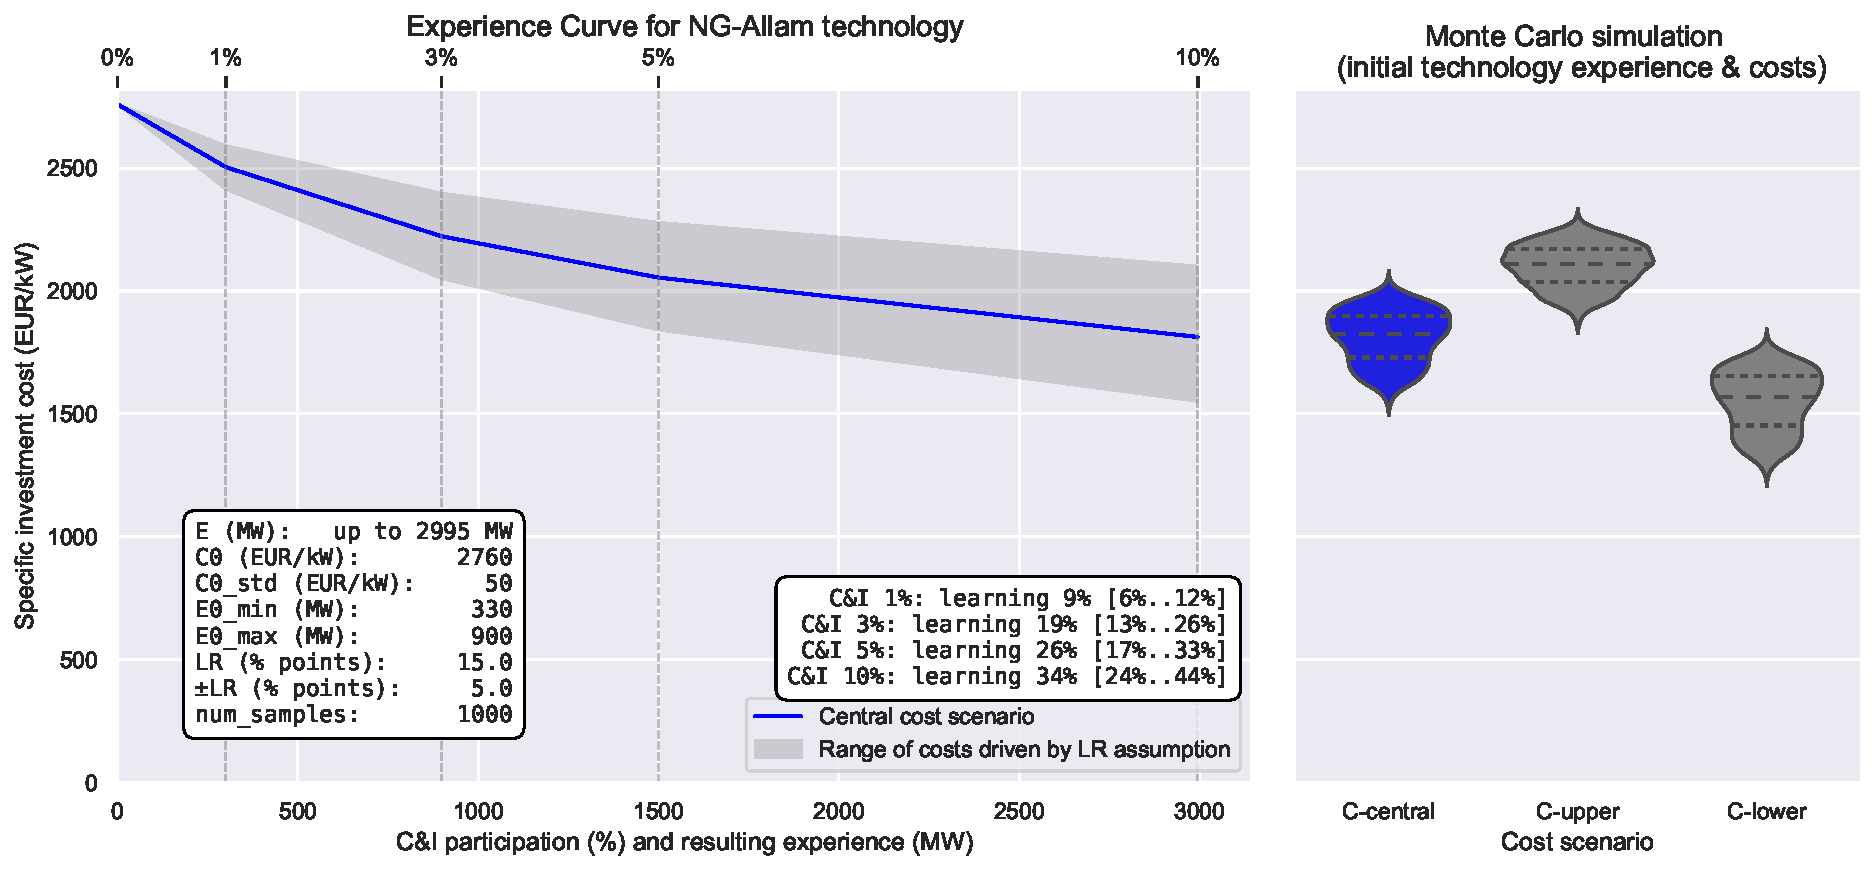
\includegraphics[width=\textwidth]{images/e_curve_NG-Allam.pdf}
    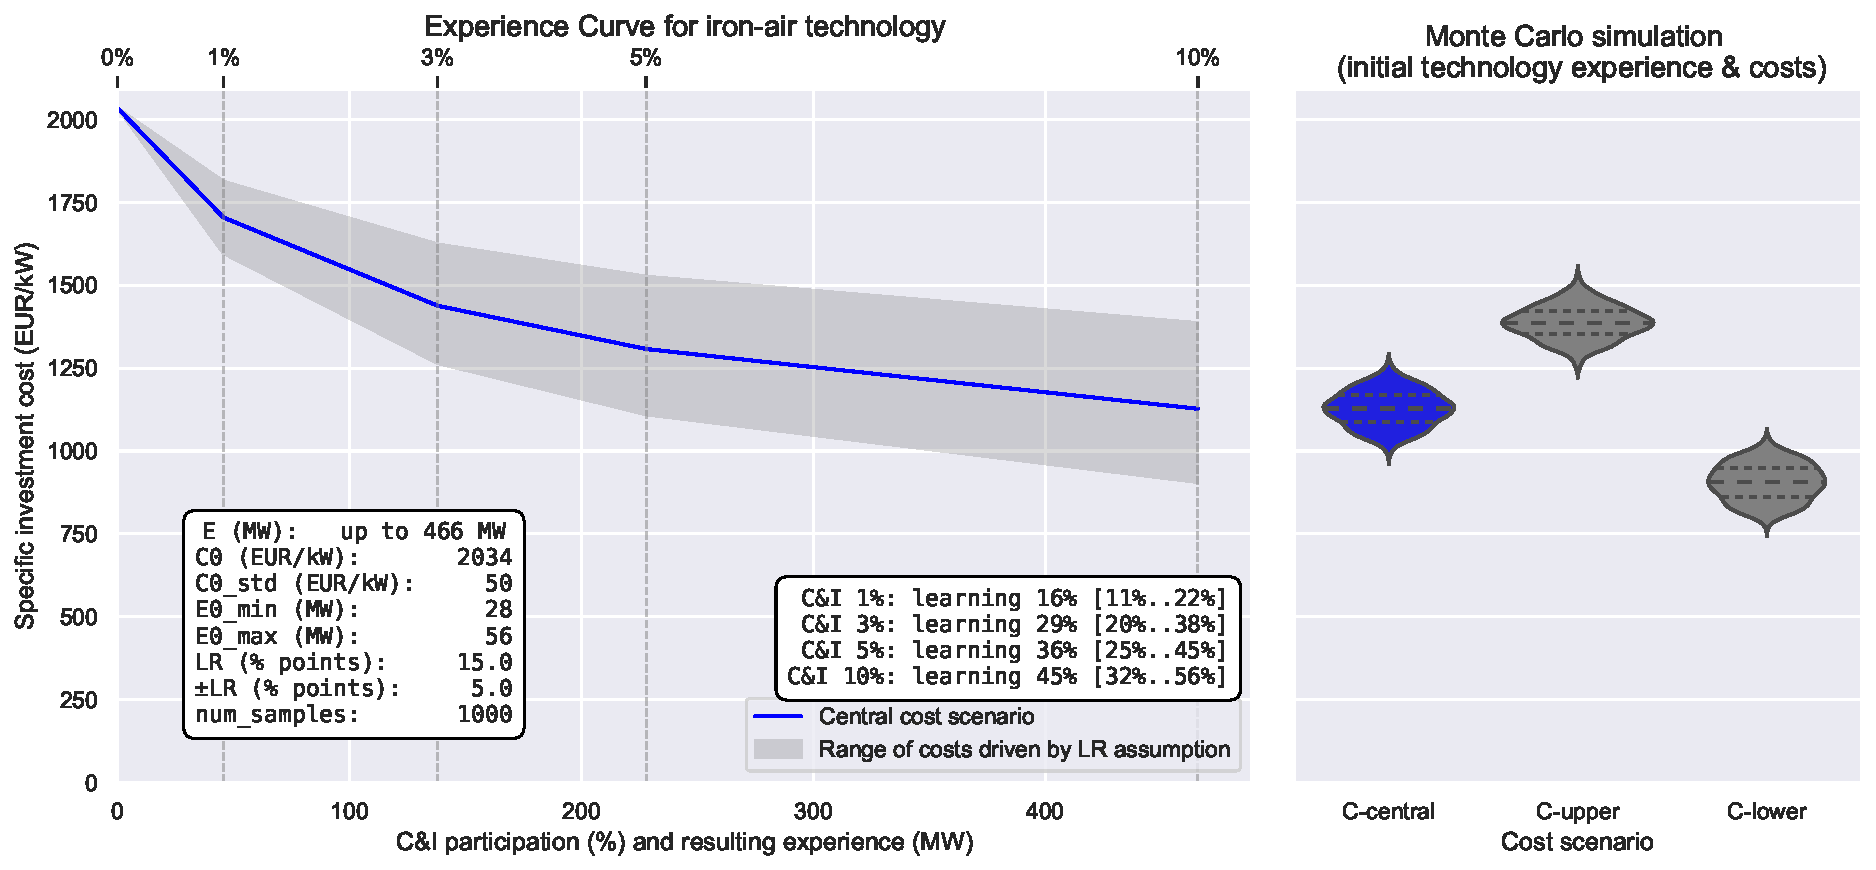
\includegraphics[width=\textwidth]{images/e_curve_iron-air.pdf}
    \caption{Technology learning curves for the NG-Allam cycle (\textbf{top panel}) and iron-air battery storage (\textbf{bottom panel}).
    The learning curves are based on the experience model with the technology investments based on 24/7 CFE model with varying C\&I participation level $[0\%..10\%]$ and learning rates of 15$\pm$5\%. \\
    For the Monte Carlo analysis calibration, the initial costs ($C0$) are sampled from a normal distribution with a mean based on our 2025 technology cost assumption and a standard deviation of 50~EUR/kW. Initial experience levels ($E0$) are sampled from a uniform distribution, with bounds derived from public information on projects planned to operate by 2025. In NG-Allam's model, initial experience lies between cases when one of three planned projects planned by 2025 is completed, and when all three projects are completed \cite{BroadwingEnergyProject, CoyoteCleanPower, FrogLakeProject}. In iron-air storage model, the distribution bounds are formed by assuming that 50\% to 100\% of the projects announced to operate by 2025 are realized on time \cite{FormEnergyLatest2024}.
    }
    \label{fig:panels}
\end{figure}

\subsection*{System impact}\label{sec3}

\comment{Here story goes as follows}

Reduced cost for advanced technologies facilitate decarbonisation of electricity systems through several channels:

First, 24/7 CFE has direct decarbonisation impact through two individual mechanisms -- profile and volume, see Priceton (2022) and Riepin \& Brown (2023) for detail. Note that profile mechanism makes 24/7 CFE impactful even in clean regions and future times.

Second, early commitments to 24/7 CFE facilitate innovation and create the early market for advanced technologies, as shown above. More companies can join 24/7 CFE movement due to reduced price premium.  This in turn lowers system emissions via the two mechanisms above.

Third, at some point, advanced technologies break even economically in the background grid, as shown in Fig. \ref{fig:impact}:

\begin{itemize}
    \item Figure shows that iron-air battery storage enters optimal investment mix with CAPEX ~1525 EUR/kW (75\% cost reduction).
    \item System emissions drop because iron-air substitute fossil peakers (gas OC), and later facilitates efficient use of RES excess.
    \item This CAPEX point is crossed if existing 2025 capacity of iron-air battery \textbf{is doubled twice}, what can be derived from Fig. \ref{fig:panels}. \\
    (here I have to simplify across multiple data points depending on realisation of E0, C0 and LR. Simply put, it needs roughly 2x expected capacity by 2025 and LR [0.10 .. 0.15].)
    \item In other words, it requires \textbf{0.35B investment} to bring iron-air experience to the point of economical break-even in the background grids by 2030. \\
    (170 MW * 2034 EUR/kW * 1e3 ) / 1e9)
    \item This learning can be reached if C\&I consumers with aggregated demand of ca. 1200MW join 24/7 CFE movement -- that is 3\% of C\&I in DE sector. NB! That learning effect can be reached with even lower participation, if C\&I consumers focus their investment strategies on LDES (iron-air).
\end{itemize}

\begin{SCfigure}[][htbp]
    \centering
    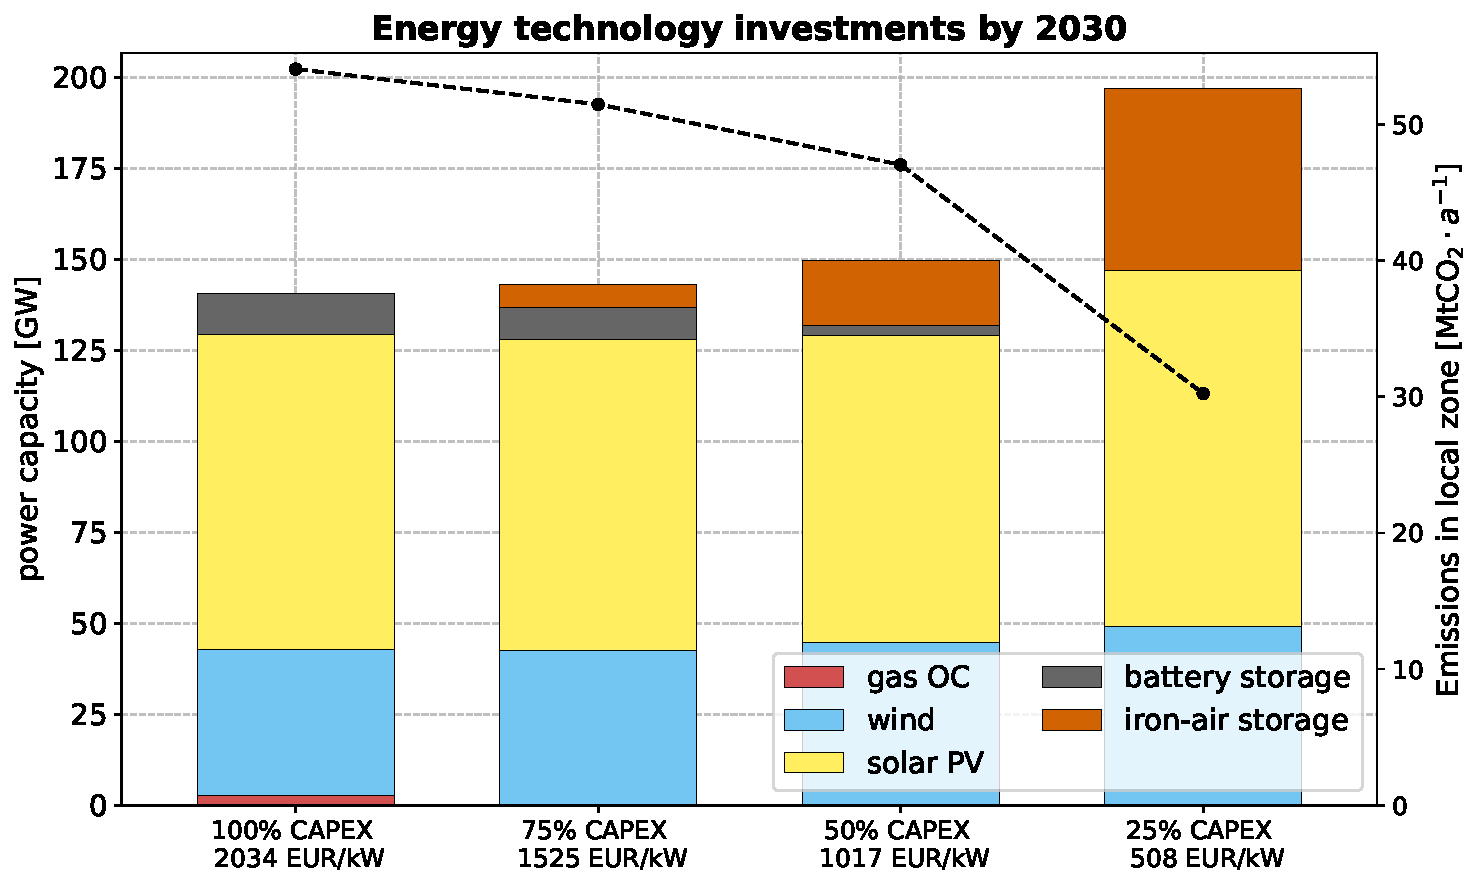
\includegraphics[width=0.65\textwidth]{images/dashboard_3.pdf}
    \caption{Power capacity investments and emissions in German 2030 electricity system as a function of CAPEX for iron-air storage. \\
    Iron-air storage has a fixed duration of 100 hours \cite{FormEnergyLatest2024}. Price for EU ETS allowances is 100 EUR/tCO$_2$. Technology costs are based on DEA \cite{DEA-technologydata}. Other background system assumptions are aligned with \citet{riepin-zenodo-systemlevel247}.}\label{fig:impact}
    \captionsetup{width=0.3\textwidth}  % Adjust according to your needs
\end{SCfigure}


\subsection*{A broad perspective}\label{sec4}

\comment{A short 1 paragraph conclusion goes as follows}

Reduced costs of advanced clean electricity technologies benefits all: \\
-- lower costs for 24/7 CFE matching for followers \\
-- makes deep decarbonization more affordable and enables more ambitious climate goals \\
-- facilitates energy security and resilience \\
-- reduce curtailment, and the need for transmission and distribution infrastructure \\


% We find that 24/7 matching is a viable and effective strategy for electricity buyers aiming to eliminate their own carbon footprint and contribute to wider system decarbonisation.
% Voluntary commitments to the hourly matching strategy have a further transformative effect on electricity systems through accelerated innovation and early deployment of advanced energy technologies

%%%%%%%%%%%%%%%%%%%%%%%%%%%%%%%%%%%%%%%%%%%%%%%%%%%%%%%%
\backmatter

\bmhead{Acknowledgements} We thank the following people for insights and fruitful discussions: Elisabeth Zeyen, Adam Forni, Brian Denvir, and the participants of the 24/7 CFE Hub Meeting in May 2024. IR acknowledges a research grant from Google LLC.

\bmhead{Author contributions} The authors contributed equally to this work.

\bmhead{Code availability} The code to reproduce the illustrative experiments is available at GitHub under open licenses \cite{code247CFE}.

\bmhead{Competing interests} \comment{I suppose there is no competing interests to declare for this work from @TUB side, TB do you agree? @DS please suggest your line here.}


%%===========================================================================================%%
%% If you are submitting to one of the Nature Portfolio journals, using the eJP submission   %%
%% system, please include the references within the manuscript file itself. You may do this  %%
%% by copying the reference list from your .bbl file, paste it into the main manuscript .tex %%
%% file, and delete the associated \verb+\bibliography+ commands.                            %%
%%===========================================================================================%%

\bibliography{sn-bibliography}% common bib file
%% if required, the content of .bbl file can be included here once bbl is generated
%%\input sn-article.bbl

\FloatBarrier

\subsection*{Technology assumptions for the illustrative example of 24/7 CFE matching}
\label{sec:annex}

\comment{Annexes are not included in Nature Comments (comments usually do not display primary research data).  Leaving this out, however, would not be scientifically rigorous, especially given the context of the comment. We can figure out some online clickable workaround if the editorial board does not like it, I'd need a quiet hour for that.}

Cost and other assumptions for energy technologies available for 24/7 CFE participating consumers are collected from the Danish Energy Agency \cite{DEA-technologydata}.
Data for advanced clean firm technologies is less reliable due to technological uncertainty and lack of commercial experience; therefore, we use publicly available information and own estimates.
A full list of technology assumptions, including the data for energy technologies in the background energy system, is available via the reproducible scientific workflow in the GitHub repository \cite{code247CFE}.

\begin{table*}[h]
    \centering
    \resizebox{\textwidth}{!}{%
        \begin{tabular}{lccccccc}
            \hline\hline
            \textbf{Technology} &
            \textbf{Year} &
            \textbf{\begin{tabular}[c]{@{}c@{}}CAPEX\\ (overnight cost)\end{tabular}} &
            \textbf{\begin{tabular}[c]{@{}c@{}}FOM\\ {[}\%/year{]}\end{tabular}} &
            \textbf{\begin{tabular}[c]{@{}c@{}}VOM\\ {[}Eur/MWh{]}\end{tabular}} &
            \textbf{\begin{tabular}[c]{@{}c@{}}Efficiency\\ {[}per unit{]}\end{tabular}} &
            \textbf{\begin{tabular}[c]{@{}c@{}}Lifetime\\ {[}years{]}\end{tabular}} &
            \textbf{Source} \\ \hline\hline
            Utility solar PV & 2025 & 612 \officialeuro/kW & 1.7 & 0.01 & - & 37.5 & \cite{DEA-technologydata} \\
            Onshore wind & 2025 & 1077 \officialeuro/kW & 1.2 & 0.015 & - & 28.5 & \cite{DEA-technologydata} \\
            Battery storage & 2025 & 187 \officialeuro/kWh & - & - & - & 22.5 & \cite{DEA-technologydata} \\
            Battery inverter & 2025 & 215 \officialeuro/kW & 0.3 & - & 0.96 & 10 & \cite{DEA-technologydata} \\
            Iron-air storage & 2025 & 2034 \officialeuro/kW$^1$ & 1 & - & 0.43$^2$ & 15 & \cite{FormEnergyLatest2024} \\
            Allam cycle generator & 2025 & 2760 \officialeuro/kW$^3$ & 14.8 & 3.2 & 0.54 & 30 & \cite{navigant-report, NetZeroAmerica-report} \\
            \hline \hline
        \end{tabular}%
    }
\begin{tablenotes}
    {\small
    \item[] Notes: $^1$iron-air storage has a fixed duration of 100h, costs comprise both power and energy components; $^2$cycle efficiency, the model factors in efficiency factor of 0.71 for charge process and 0.60 for discharge; $^3$costs also include estimate of 40 \officialeuro/tCO$_2$ for carbon transport and sequestration; all costs are in 2023 euros; CAPEX = capital expenditure; FOM = fixed operations and maintenance costs; VOM = variable operations and maintenance costs.
    }
\end{tablenotes}
    \vspace{0.2cm}
    \caption{Technology assumptions.}
    \label{tab:tech_costs}
\end{table*}

\end{document}
